\documentclass[11pt, a4paper]{article}

\usepackage[utf8]{inputenc}
\usepackage[T1]{fontenc}
\usepackage{lmodern}
\usepackage[margin=2.4cm]{geometry}
\usepackage{microtype}
\usepackage{graphicx}
\usepackage{booktabs}
\usepackage{array}
\usepackage{multirow}
\usepackage{makecell}
\usepackage{caption}
\usepackage{subcaption}
\usepackage{xcolor}
\usepackage{titlesec}
\usepackage{enumitem}
\usepackage{amsmath, amssymb}
\usepackage{hyperref}
\hypersetup{
  colorlinks=true,
  linkcolor=black,
  citecolor=blue!50!black,
  urlcolor=blue!50!black,
}
\usepackage{fancyhdr}
\usepackage{siunitx}
\sisetup{detect-all, table-format=1.4}

\pagestyle{fancy}
\fancyhf{}
\rhead{\small FEELIN Phase 2 Wrap-up Report}
\lhead{\small 2026-06-01}
\rfoot{\thepage}

\titleformat{\section}{\large\bfseries}{\thesection}{0.6em}{}
\titleformat{\subsection}{\normalsize\bfseries}{\thesubsection}{0.5em}{}

\setlength{\parskip}{6pt}
\setlength{\parindent}{0pt}

\newcommand{\fefn}[1]{\texttt{\small #1}}
\newcommand{\eg}{e.g.,\ }
\newcommand{\ie}{i.e.,\ }

\title{\vspace{-2em}\textbf{Training Paradigms on Frozen Brain Foundation Features for
       Naturalistic Emotion Prediction}}
\author{Seokjin Moon \\
        \small Department of Brain and Cognitive Sciences, Seoul National University}
\date{2026-06-01}

\begin{document}
\maketitle
\thispagestyle{fancy}

\begin{abstract}
\noindent
Frozen probes on brain foundation model (BFM) features set the brain-only ceiling for
naturalistic emotion prediction at roughly $0.74$ AUROC for valence-extreme classification
and $0.32$ Pearson $r$ for valence regression on the Horikawa five-subject corpus, with
the corresponding video-only baseline (a pretrained image-text encoder) reaching $0.97$
and $0.76$. We ask whether brain emotion prediction can be moved beyond this brain-only
ceiling by training, holding the brain feature extractor frozen and varying only the
downstream training paradigm. We evaluate eight downstream paradigms organised in two
groups. Four brain-only paradigms train a small head on the brain feature alone
(supervised multilayer perceptron (MLP), video-feature distillation, multitask with a
video reconstruction auxiliary head, and a per-subject identity embedding). Four joint
paradigms ingest both brain and video features (late linear fusion, multi-head
self-attention with a learned class token, bidirectional brain-video cross-attention, and
contrastive alignment followed by a probe). All eight paradigms share an identical
five-fold stimulus-stratified protocol on four emotion tasks (valence and arousal, each as
extreme-quartile binary and continuous regression). None of the four brain-only paradigms
moves the brain-only ceiling above the frozen-probe baseline. The four joint paradigms,
in contrast, recover and in two of four tasks slightly exceed the video-only ceiling
without losing the brain-side contribution. Within the joint group, the choice of fusion
matters task by task. Late linear fusion attains the best classification number, whereas
token-attention dominates the regression tasks by an absolute margin. The contrastive
brain branch, evaluated alone after alignment, underperforms every other brain-only
paradigm, indicating that an alignment objective designed to compress shared structure
can erode the emotion-relevant signal on the brain side. We discuss the implications for
how naturalistic-emotion BFM benchmarks should report joint and brain-only numbers.
\end{abstract}

\section{Introduction}

The companion Phase 1 benchmark established the frozen-probe ceiling for naturalistic
emotion fMRI on the Horikawa five-subject corpus across three brain foundation models
(SwiFT, Brain-JEPA, NeuroSTORM), a 450-region atlas baseline, and five pretrained video
encoders, all evaluated under a single five-fold stimulus-stratified protocol. Two facts
from that benchmark set up the present report. First, the brain-only ceiling on
valence-extreme classification under frozen probing is approximately $0.74$ AUROC, with
the corresponding video-only ceiling at $0.97$ for an image-text contrastive encoder.
Second, the gap between brain-only and video-only is consistent across tasks (binary and
continuous, valence and arousal), and is not removed by switching probe head or training
mode within the frozen-probe family.

The natural next question is whether training, applied at the level of the downstream
head rather than the brain encoder, can move the brain side of this ceiling. Two
hypotheses motivate this question. The first is that the small per-subject sample size
(roughly $1135$ for binary tasks and $2185$ for regression, distributed across five
subjects) is the binding constraint, and that paradigm choice does not matter. The second
is that a training paradigm that introduces information beyond the per-stimulus emotion
target, such as distillation from a stronger video feature or an auxiliary
video-reconstruction loss, could push the brain-only number higher even with the brain
encoder frozen. We test eight paradigms in a controlled way to distinguish these
hypotheses, and we further ask whether a joint paradigm that uses both brain and video
inputs can do better than the video-only baseline, which is the relevant ceiling for any
future model proposed to integrate brain and stimulus in this regime.

This report contributes the following.

\begin{enumerate}[leftmargin=1.4em, itemsep=2pt]
  \item A controlled four-by-four paradigm benchmark on the same Horikawa five-subject
        corpus and the same four-task protocol used in Phase 1, with brain features held
        frozen and only the downstream paradigm varied. The brain encoder is Brain-JEPA,
        which is the most defensible default identified in Phase 1.
  \item A direct comparison of best Phase 2 paradigm against best Phase 1 frozen-probe
        condition per task, decomposed into a brain-only subcomparison and a joint
        subcomparison.
  \item An observation that the four brain-only paradigms collapse onto the frozen-probe
        ceiling regardless of training signal, while the joint paradigms separate into a
        regression-strong family (token attention) and a classification-strong family
        (late linear fusion).
  \item An observation that the contrastive alignment paradigm, evaluated on its
        brain-only branch after alignment, underperforms every other brain-only paradigm.
\end{enumerate}

The methods are described in Section~\ref{sec:methods}. Results follow in
Section~\ref{sec:results}. Section~\ref{sec:discussion} discusses interpretation and the
implications for joint brain-video models, including the BrainVLM follow-up.

\section{Methods}
\label{sec:methods}

\subsection{Dataset and protocol}
We use the Horikawa naturalistic emotion fMRI corpus, five subjects who viewed $2185$
short video clips during 3T fMRI scanning. Each clip carries a continuous self-rated
valence and arousal score on a $[1, 5]$ scale. The four emotion tasks are the same as in
Phase 1. The binary tasks restrict to extreme-quartile stimuli and predict the
high-quartile membership ($N_{\text{stim}} = 1135$). The regression tasks use all $2185$
stimuli with the continuous score as target. Evaluation is five-fold
stimulus-stratified cross-validation, with three random training seeds per fold for
neural paradigms and a single seed for the closed-form late-fusion baseline. Main metrics
are AUROC (binary) and Pearson $r$ (regression).

\subsection{Frozen feature inputs}
The brain feature is the per-stimulus pooled output of frozen Brain-JEPA with
\fefn{resting} initialisation and zero temporal padding to the model's native input
length. This is the brain-only condition with the highest Phase 1 ceiling among the three
benchmarked BFMs. The video feature is the per-stimulus output of frozen CLIP
(\fefn{openai/clip-vit-large-patch14}). Both are loaded from the Phase 1 feature cache
under \fefn{output/embeddings/\{brain\_jepa,clip\}/}. Each feature is centred and
standardised per training fold using statistics computed on the training subset only.

\subsection{Architecture overview}
Figure~\ref{fig:arch} shows the eight paradigms on one canvas. The top row contains the
four joint paradigms (A token-attention, B cross-attention, C contrastive alignment, D
late linear fusion), each ingesting both brain and video features. The bottom row
contains the four brain-only paradigms (I supervised multilayer perceptron (MLP), II
distillation, III multitask, IV subject-aware), each ingesting only the brain feature at
inference. Video appears as a teacher signal in II and as a reconstruction target in III,
but is never present at inference time for any brain-only paradigm.

\begin{figure}[h]
\centering
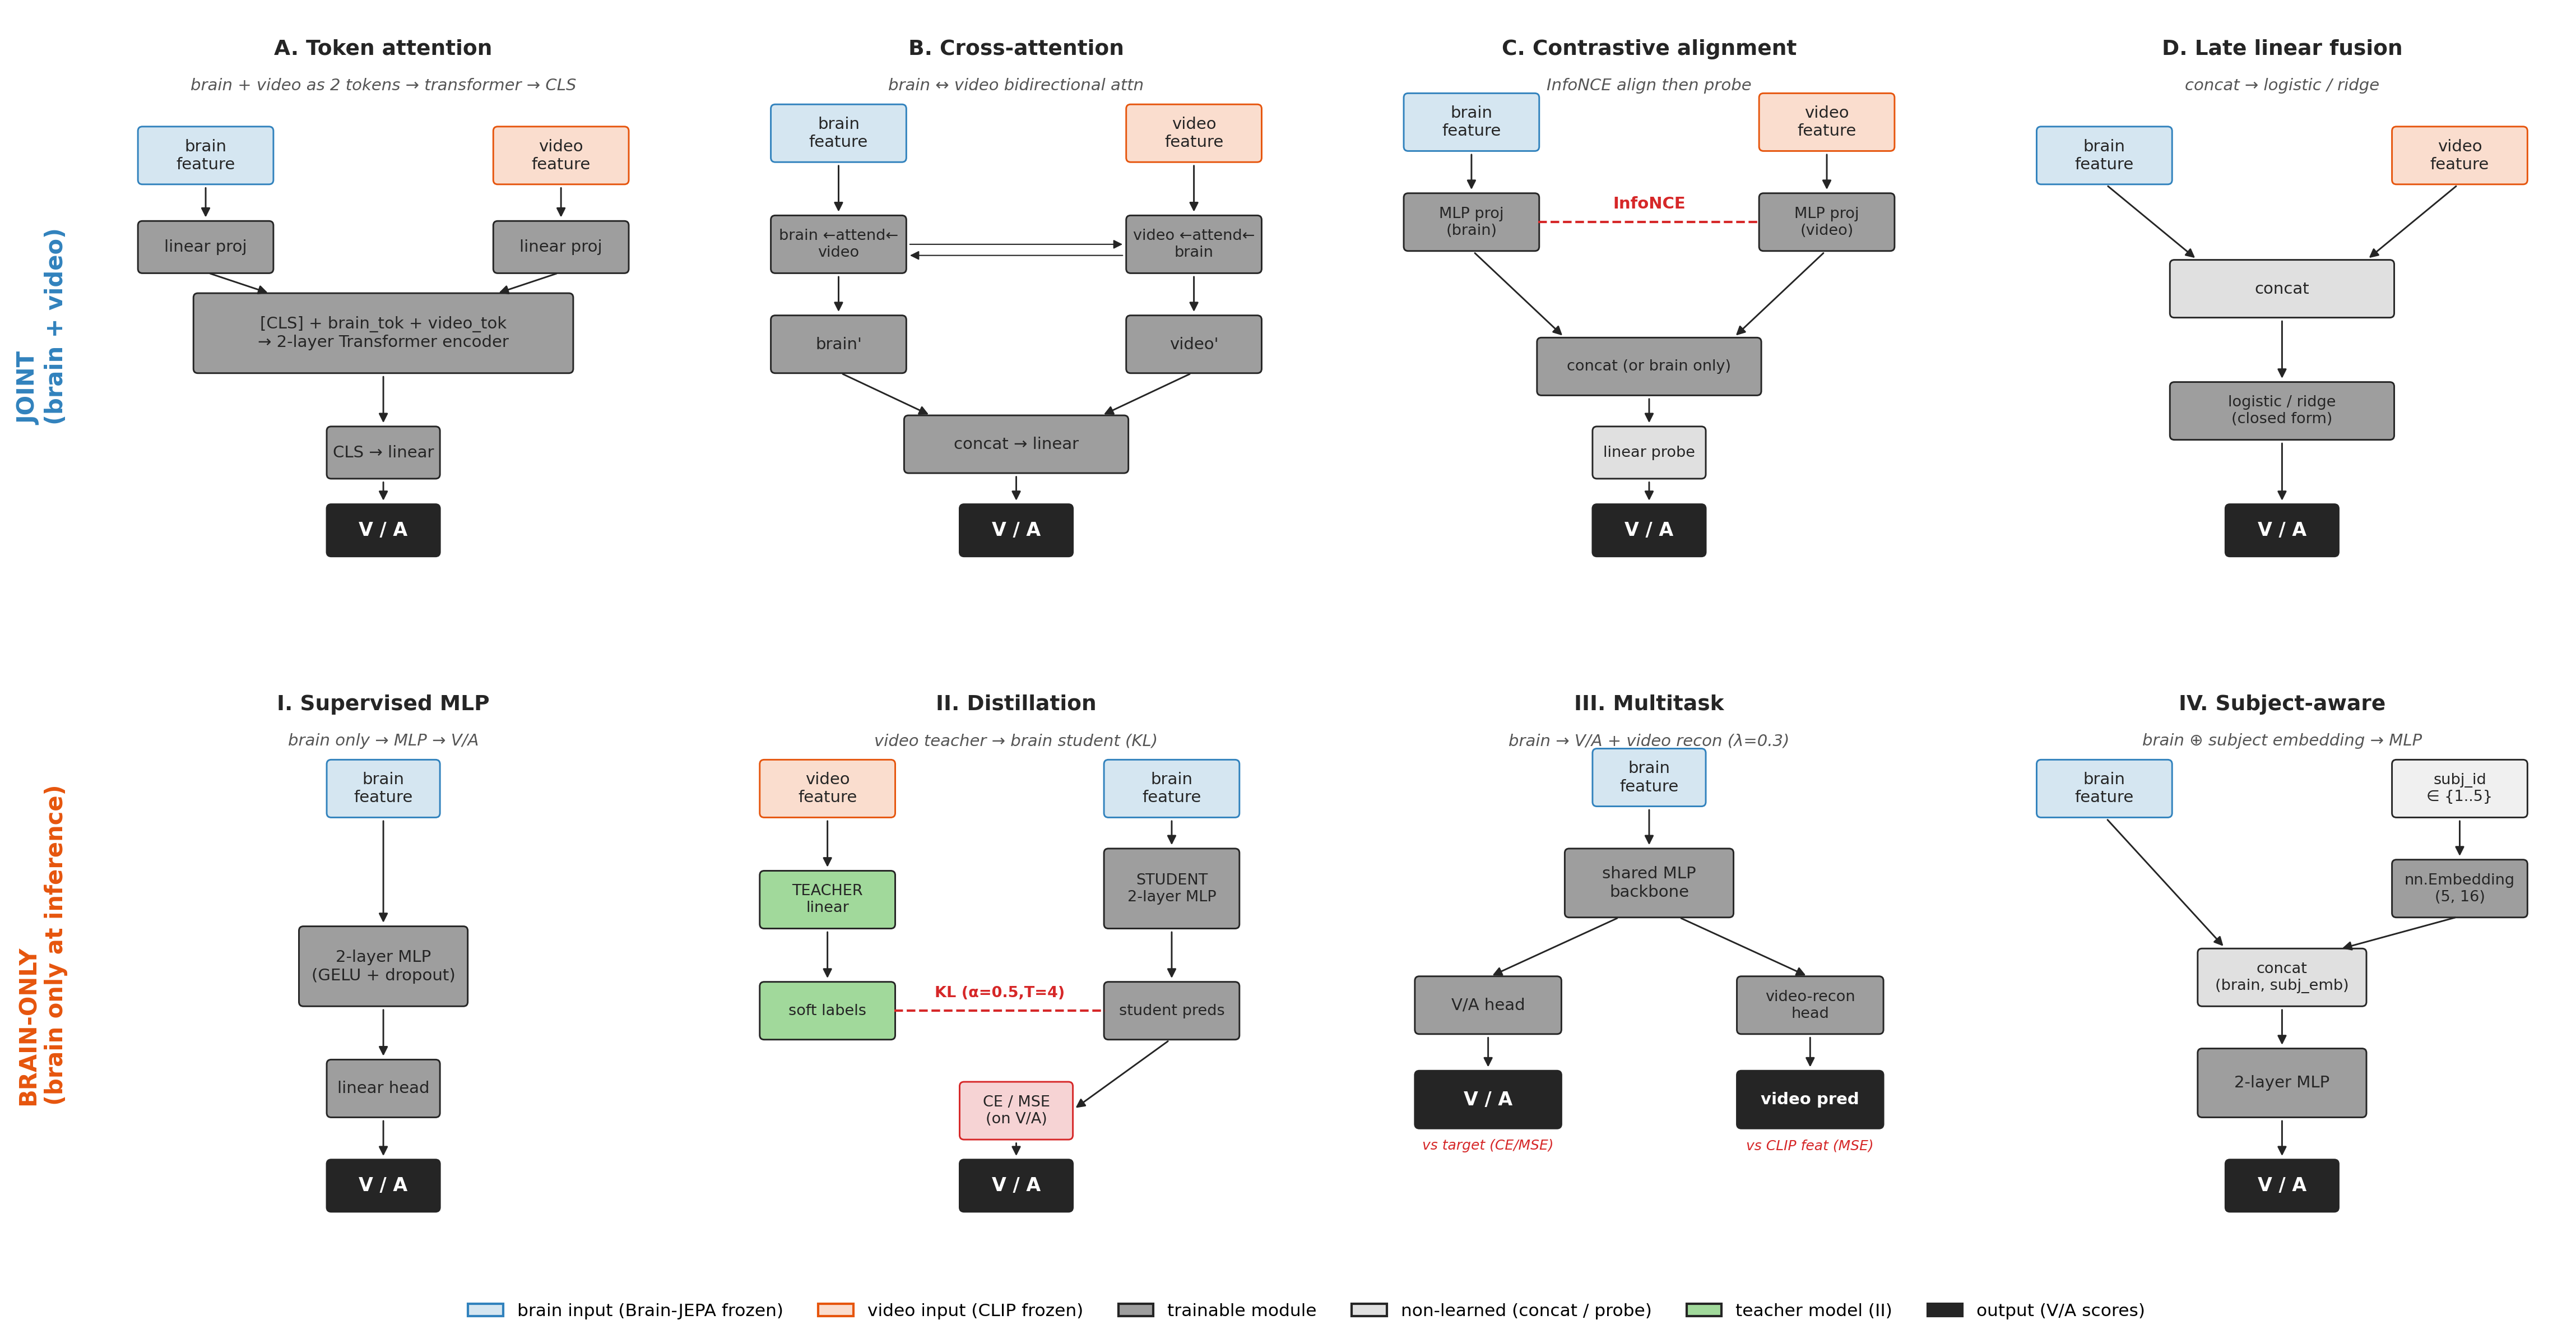
\includegraphics[width=\linewidth]{figs/architecture_8methods.png}
\caption{The eight Phase 2 paradigms. Top row, joint paradigms take both brain and video
features as input. Bottom row, brain-only paradigms take only the brain feature as input
at inference, although video appears as a teacher signal in II and as a reconstruction
target in III. Trainable blocks are shaded grey. The brain encoder (Brain-JEPA) and the
video encoder (CLIP) are frozen for all eight paradigms.}
\label{fig:arch}
\end{figure}

\subsection{Brain-only paradigms (I to IV)}
All four brain-only paradigms take the same per-stimulus brain feature as input and emit
a per-stimulus prediction of the four targets. They differ only in the training signal.

\begin{description}[leftmargin=1.4em, itemsep=2pt]
  \item[Paradigm~I, supervised MLP.] A two-layer MLP head with GELU and dropout, trained
        directly on the emotion target using binary cross-entropy or mean squared error.
        This is the strict supervised baseline.
  \item[Paradigm~II, video-feature distillation.] A two-layer MLP brain student trained
        with a convex combination of the supervised target loss and a Kullback-Leibler
        distillation loss against a closed-form CLIP teacher fit on the same fold, with
        teacher temperature $T = 4$ and student weight $\alpha = 0.5$. The teacher is
        precomputed per fold from frozen CLIP features.
  \item[Paradigm~III, multitask with video reconstruction.] A shared two-layer backbone
        is followed by two heads, the emotion target head and a video-feature
        reconstruction head, with reconstruction loss weight $\lambda = 0.3$. The
        reconstruction target is the corresponding fold-normalised CLIP feature.
  \item[Paradigm~IV, per-subject identity.] A 16-dimensional learned subject embedding is
        concatenated with the brain feature before the same MLP head as in Paradigm~I.
        The embedding is trained jointly with the head.
\end{description}

All four use the same hyperparameter grid (learning rate $\{10^{-4}, 3\times10^{-4},
10^{-3}, 3\times10^{-3}, 10^{-2}\}$ with cosine decay, AdamW, early stopping on validation
main metric). Each paradigm is run for three random training seeds per fold, with a
divergence guard (NaN check plus gradient clipping at $\|\cdot\|_2 = 1$) that retries with
the next learning rate if the current run diverges.

\subsection{Joint paradigms (A to D)}
The joint paradigms ingest both the brain feature and the video feature.

\begin{description}[leftmargin=1.4em, itemsep=2pt]
  \item[Paradigm~A, token attention.] Brain and video features are projected to a common
        dimension, prepended with a learned class token, augmented with a learned modality
        type embedding, and processed by a two-layer multi-head self-attention encoder.
        The class token logit is the readout. This is the closest to a generic Transformer
        late-fusion design.
  \item[Paradigm~B, brain-video cross-attention.] A symmetric cross-attention module
        updates the brain representation conditional on video and the video representation
        conditional on brain, with two layers and residual connections. The brain-side
        output is the readout.
  \item[Paradigm~C, contrastive alignment.] Brain and video features are projected by
        two-layer MLPs to a shared $D = 256$ embedding space, and the two projections are
        trained with a symmetric InfoNCE loss with learnable temperature, no emotion
        supervision during alignment. After alignment, a linear probe is fit on the
        aligned features. We report two readouts in Section~\ref{sec:results}: the joint
        readout uses both branches concatenated; the brain-only readout uses only the
        aligned brain branch.
  \item[Paradigm~D, late linear fusion.] The brain and video features are concatenated
        and processed by a closed-form linear classifier (logistic regression for binary,
        ridge for regression), with the regularisation strength selected on validation.
        This is the standard sklearn-based late fusion and serves as the simplest joint
        baseline.
\end{description}

Paradigms A and B share an identical training recipe with the brain-only paradigms
(AdamW, cosine schedule, three seeds per fold, divergence guard). Paradigm~D is closed
form and runs once per fold. Paradigm~C runs three seeds for alignment, and the probe is
re-fit per seed.

\subsection{What is and is not varied}
The brain encoder, video encoder, fold definitions, target standardisation, and four-task
protocol are all identical to Phase 1. Only the downstream paradigm changes. This isolates
paradigm effect from feature-extraction effect, and it ensures every Phase 2 number is
directly comparable to the Phase 1 frozen-probe table for the same task.

\section{Results}
\label{sec:results}

\subsection{Per-task numbers across all eight paradigms}
Table~\ref{tab:per-task} reports the test main metric mean and standard deviation across
folds and seeds for each of the eight paradigms on each of the four tasks.

\begin{table}[h]
\centering
\caption{Per-task test main metric for the eight Phase 2 paradigms, mean and standard
deviation across five folds and three seeds (Paradigm~D is closed-form, five folds and
one seed). \textbf{Bold} denotes the best paradigm per task. Lower block lists the four
brain-only paradigms; upper block lists the four joint paradigms.}
\label{tab:per-task}
\small
\begin{tabular}{l S S S S}
\toprule
Paradigm & {V\_binary AUROC} & {A\_binary AUROC} & {V\_reg $r$} & {A\_reg $r$} \\
\midrule
A token-attention      & 0.9670 (0.0111) & 0.7919 (0.0482) & \textbf{0.7628 (0.0209)} & \textbf{0.4241 (0.0500)} \\
B cross-attention      & 0.9663 (0.0087) & 0.7863 (0.0539) & 0.7454 (0.0229) & 0.3956 (0.0442) \\
C contrastive (joint)  & 0.9606 (0.0084) & 0.7699 (0.0438) & 0.7123 (0.0217) & 0.3522 (0.0505) \\
D late linear fusion   & \textbf{0.9718 (0.0082)} & \textbf{0.8025 (0.0528)} & 0.5888 (0.0246) & 0.2682 (0.0404) \\
\midrule
I supervised MLP       & 0.7165 (0.0192) & 0.6534 (0.0274) & 0.3238 (0.0200) & 0.2262 (0.0326) \\
II distillation        & 0.7214 (0.0186) & 0.6645 (0.0299) & 0.3224 (0.0217) & 0.2296 (0.0330) \\
III multitask          & 0.7235 (0.0209) & 0.6573 (0.0273) & 0.3254 (0.0169) & 0.2275 (0.0341) \\
IV subject-aware       & 0.7206 (0.0172) & 0.6536 (0.0266) & 0.3225 (0.0181) & 0.2256 (0.0330) \\
\midrule
C contrastive (brain)  & 0.7123 (0.0137) & 0.6485 (0.0302) & 0.2950 (0.0186) & 0.2208 (0.0326) \\
\bottomrule
\end{tabular}
\end{table}

Three observations follow directly from the table. First, the four brain-only paradigms
cluster tightly within each task. The maximum spread between the strongest and weakest
brain-only paradigm is $0.0070$ AUROC on V\_binary, $0.0111$ on A\_binary, $0.0030$ Pearson
$r$ on V\_reg, and $0.0040$ on A\_reg. These spreads are smaller than the standard
deviation across folds and seeds, so no brain-only paradigm is meaningfully ahead of any
other. Second, the contrastive brain-only readout (Paradigm~C with the joint branch
discarded) is consistently the lowest brain-side number on every task. The gap to the
strongest brain-only paradigm is $0.0112$ AUROC on V\_binary, $0.0160$ on A\_binary,
$0.0304$ Pearson $r$ on V\_reg, and $0.0088$ on A\_reg. Third, every joint paradigm is
above every brain-only paradigm on every task, and the absolute gap is large.

\subsection{Joint paradigms versus the video-only Phase 1 ceiling}
We next compare the best Phase 2 paradigm per task against the best Phase 1 frozen-probe
condition per task. The Phase 1 top is dominated by the CLIP frozen probe, so the
relevant comparison is whether adding the brain feature on top of CLIP either preserves
or improves over the CLIP-only number. Table~\ref{tab:phase1cmp} reports this comparison.

\begin{table}[h]
\centering
\caption{Best Phase 2 paradigm per task against the best Phase 1 frozen-probe per task.
The delta column is positive when Phase 2 beats Phase 1, negative when Phase 1 is
stronger. Numbers are mean across folds and seeds.}
\label{tab:phase1cmp}
\small
\begin{tabular}{l l S l S S}
\toprule
Task & Phase 2 best & {Phase 2} & Phase 1 best & {Phase 1} & {$\Delta$} \\
\midrule
V\_binary & D late fusion       & 0.9718 & CLIP (linear) & 0.9708 & 0.0010 \\
A\_binary & D late fusion       & 0.8025 & CLIP (linear) & 0.8003 & 0.0022 \\
V\_reg    & A token-attention   & 0.7628 & CLIP (linear) & 0.7651 & -0.0023 \\
A\_reg    & A token-attention   & 0.4241 & CLIP (linear) & 0.4232 & 0.0009 \\
\bottomrule
\end{tabular}
\end{table}

On three of four tasks the best Phase 2 paradigm narrowly exceeds the best Phase 1
condition, and on V\_reg the best Phase 2 paradigm is $0.0023$ below it. The absolute
margins are small in all four cases and are within the across-fold variability reported
in Table~\ref{tab:per-task}. We do not claim that adding the brain feature on top of CLIP
improves on the CLIP-only baseline. The relevant interpretation is the symmetric one,
that the joint paradigms recover the CLIP ceiling and do not lose the brain-side
contribution. Section~\ref{sec:discussion} returns to this point.

\subsection{Joint versus brain-only summary}
Figure~\ref{fig:jb} summarises the per-task comparison of the best joint paradigm against
the best brain-only paradigm. The gap is large in absolute terms and consistent in sign
across the four tasks. The gap is widest on V\_reg ($\Delta = 0.4374$ Pearson $r$) and
narrowest on A\_binary ($\Delta = 0.1380$ AUROC).

\begin{figure}[h]
\centering
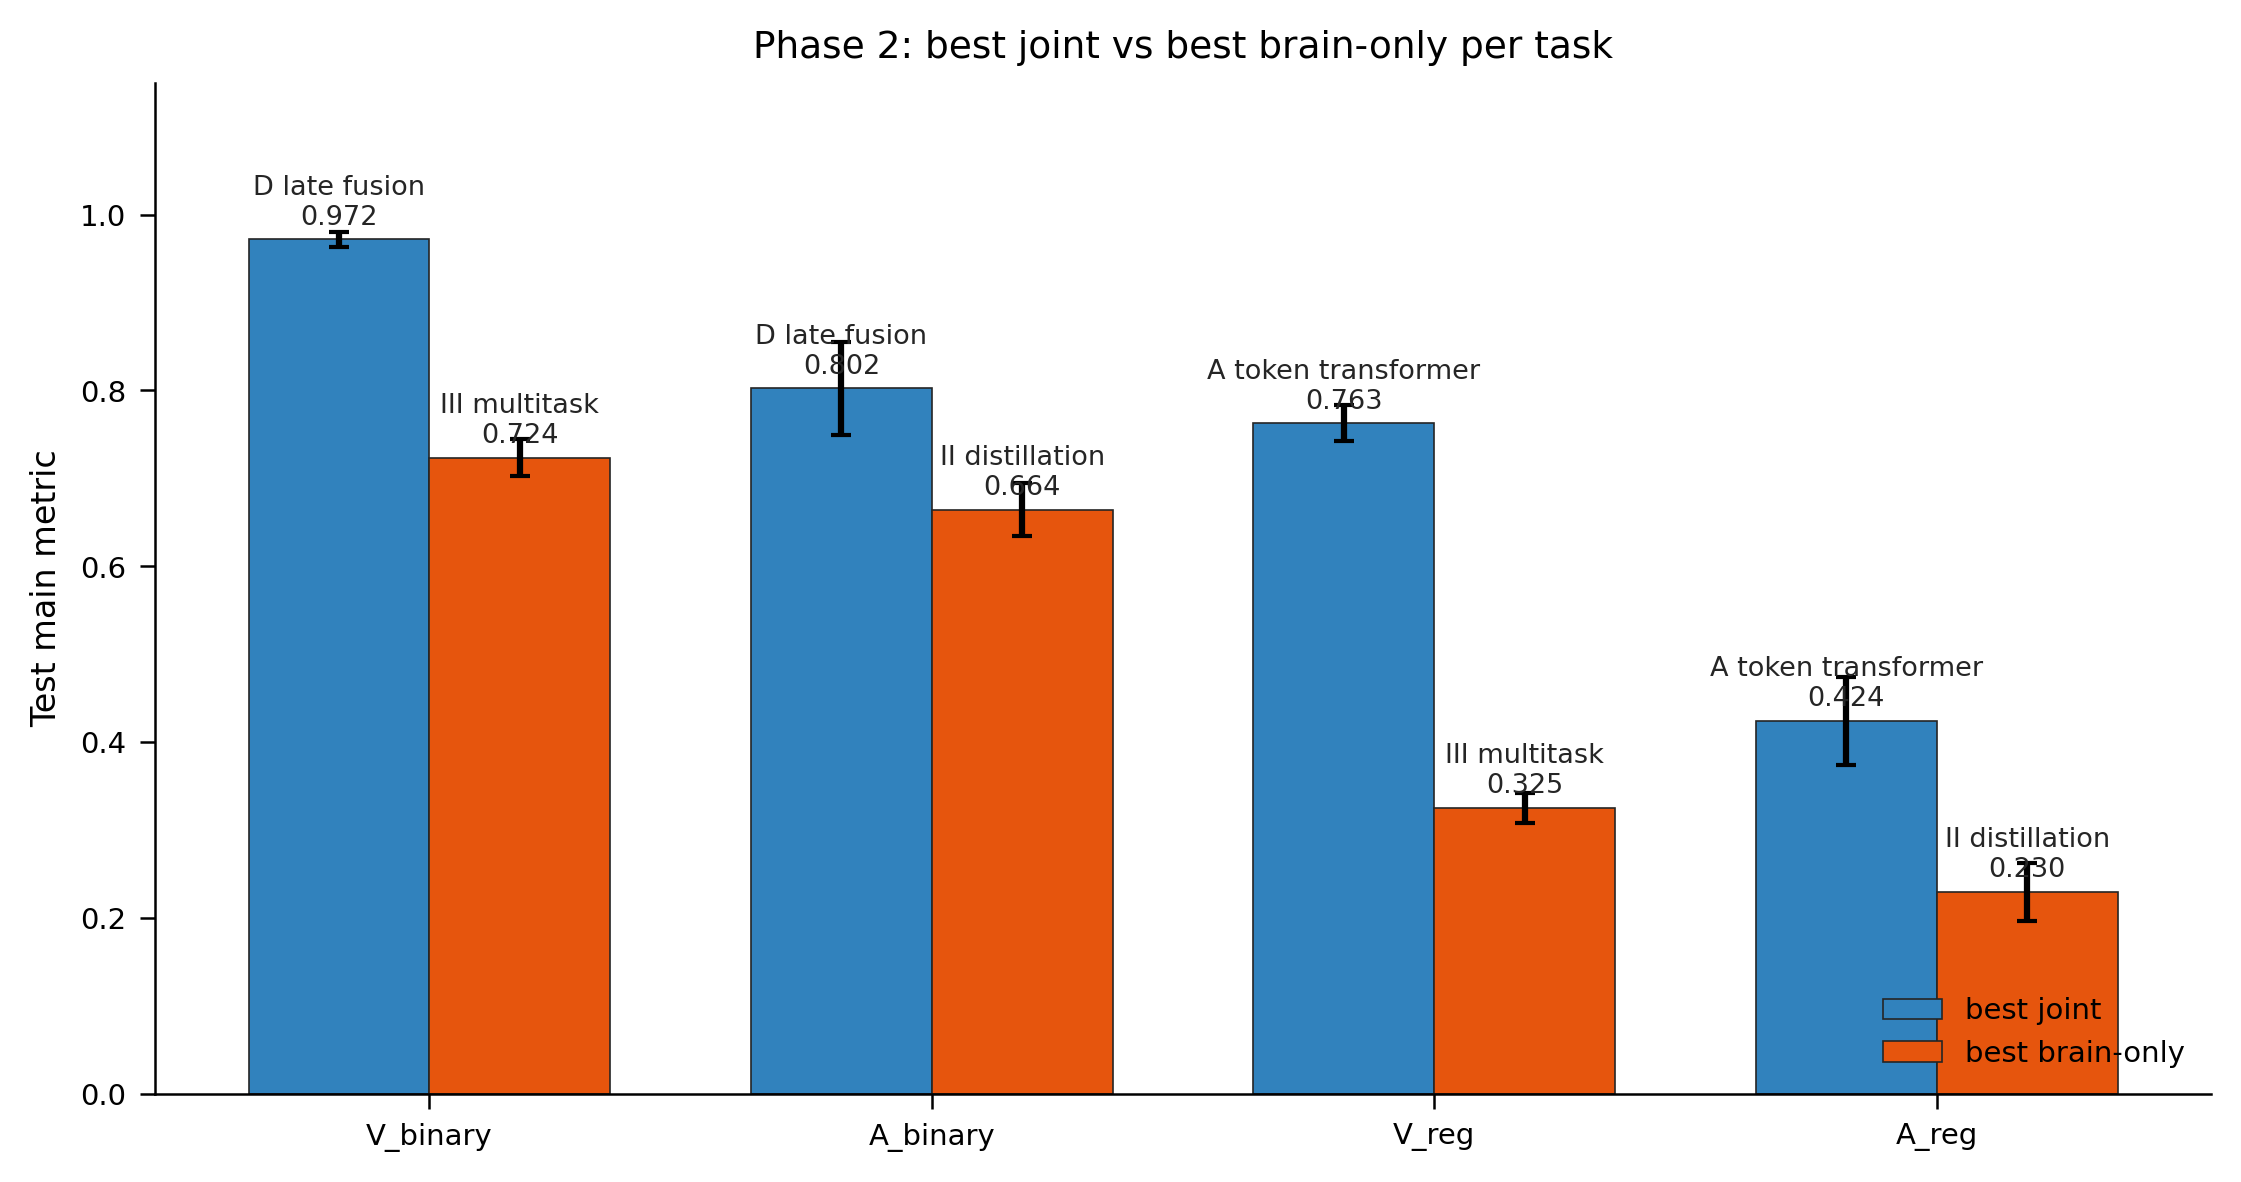
\includegraphics[width=0.82\linewidth]{figs/joint_vs_brainonly.png}
\caption{Best joint paradigm against best brain-only paradigm per task. Error bars denote
across-fold standard deviation of the best paradigm. The annotation above each bar is the
paradigm name selected as best.}
\label{fig:jb}
\end{figure}

\subsection{Per-task ranking with Phase 1 reference lines}
Figure~\ref{fig:ranking} shows the per-task ranking of all eight Phase 2 paradigms (with
the contrastive brain-only readout shown as a separate row). The dashed horizontal line
marks the Phase 1 top-overall condition and the dotted line marks the Phase 1 top-BFM
condition. The figure shows that the joint paradigms reach the dashed line, while the
brain-only paradigms hover at the dotted line.

\begin{figure}[h]
\centering
\begin{subfigure}{0.48\linewidth}
  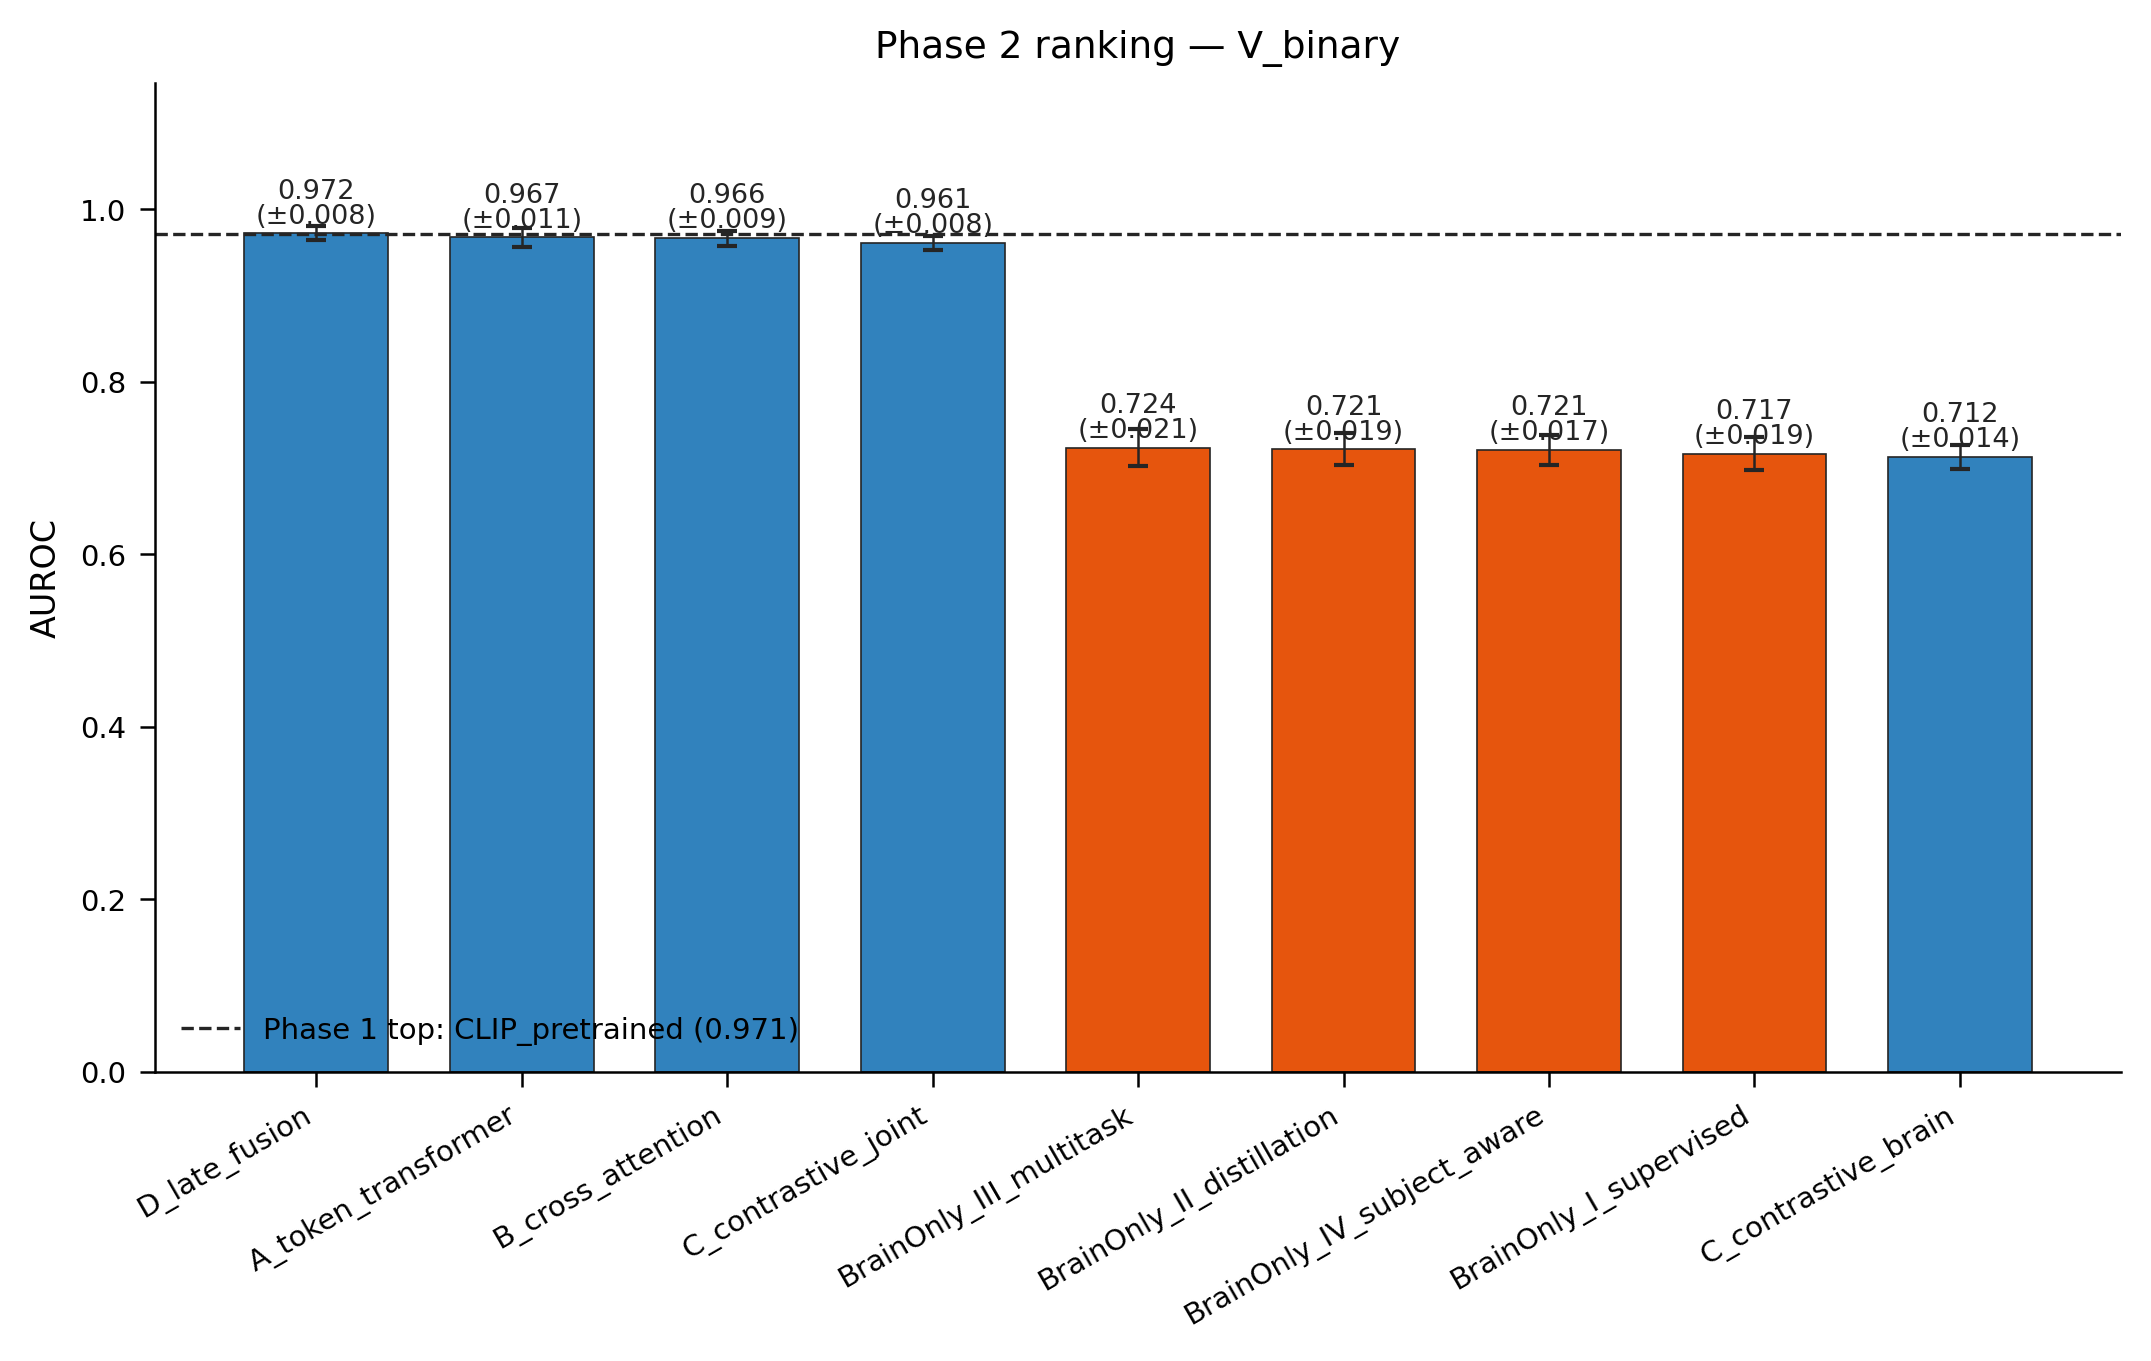
\includegraphics[width=\linewidth]{figs/ranking_V_binary.png}
  \caption{V\_binary, AUROC.}
\end{subfigure}
\hfill
\begin{subfigure}{0.48\linewidth}
  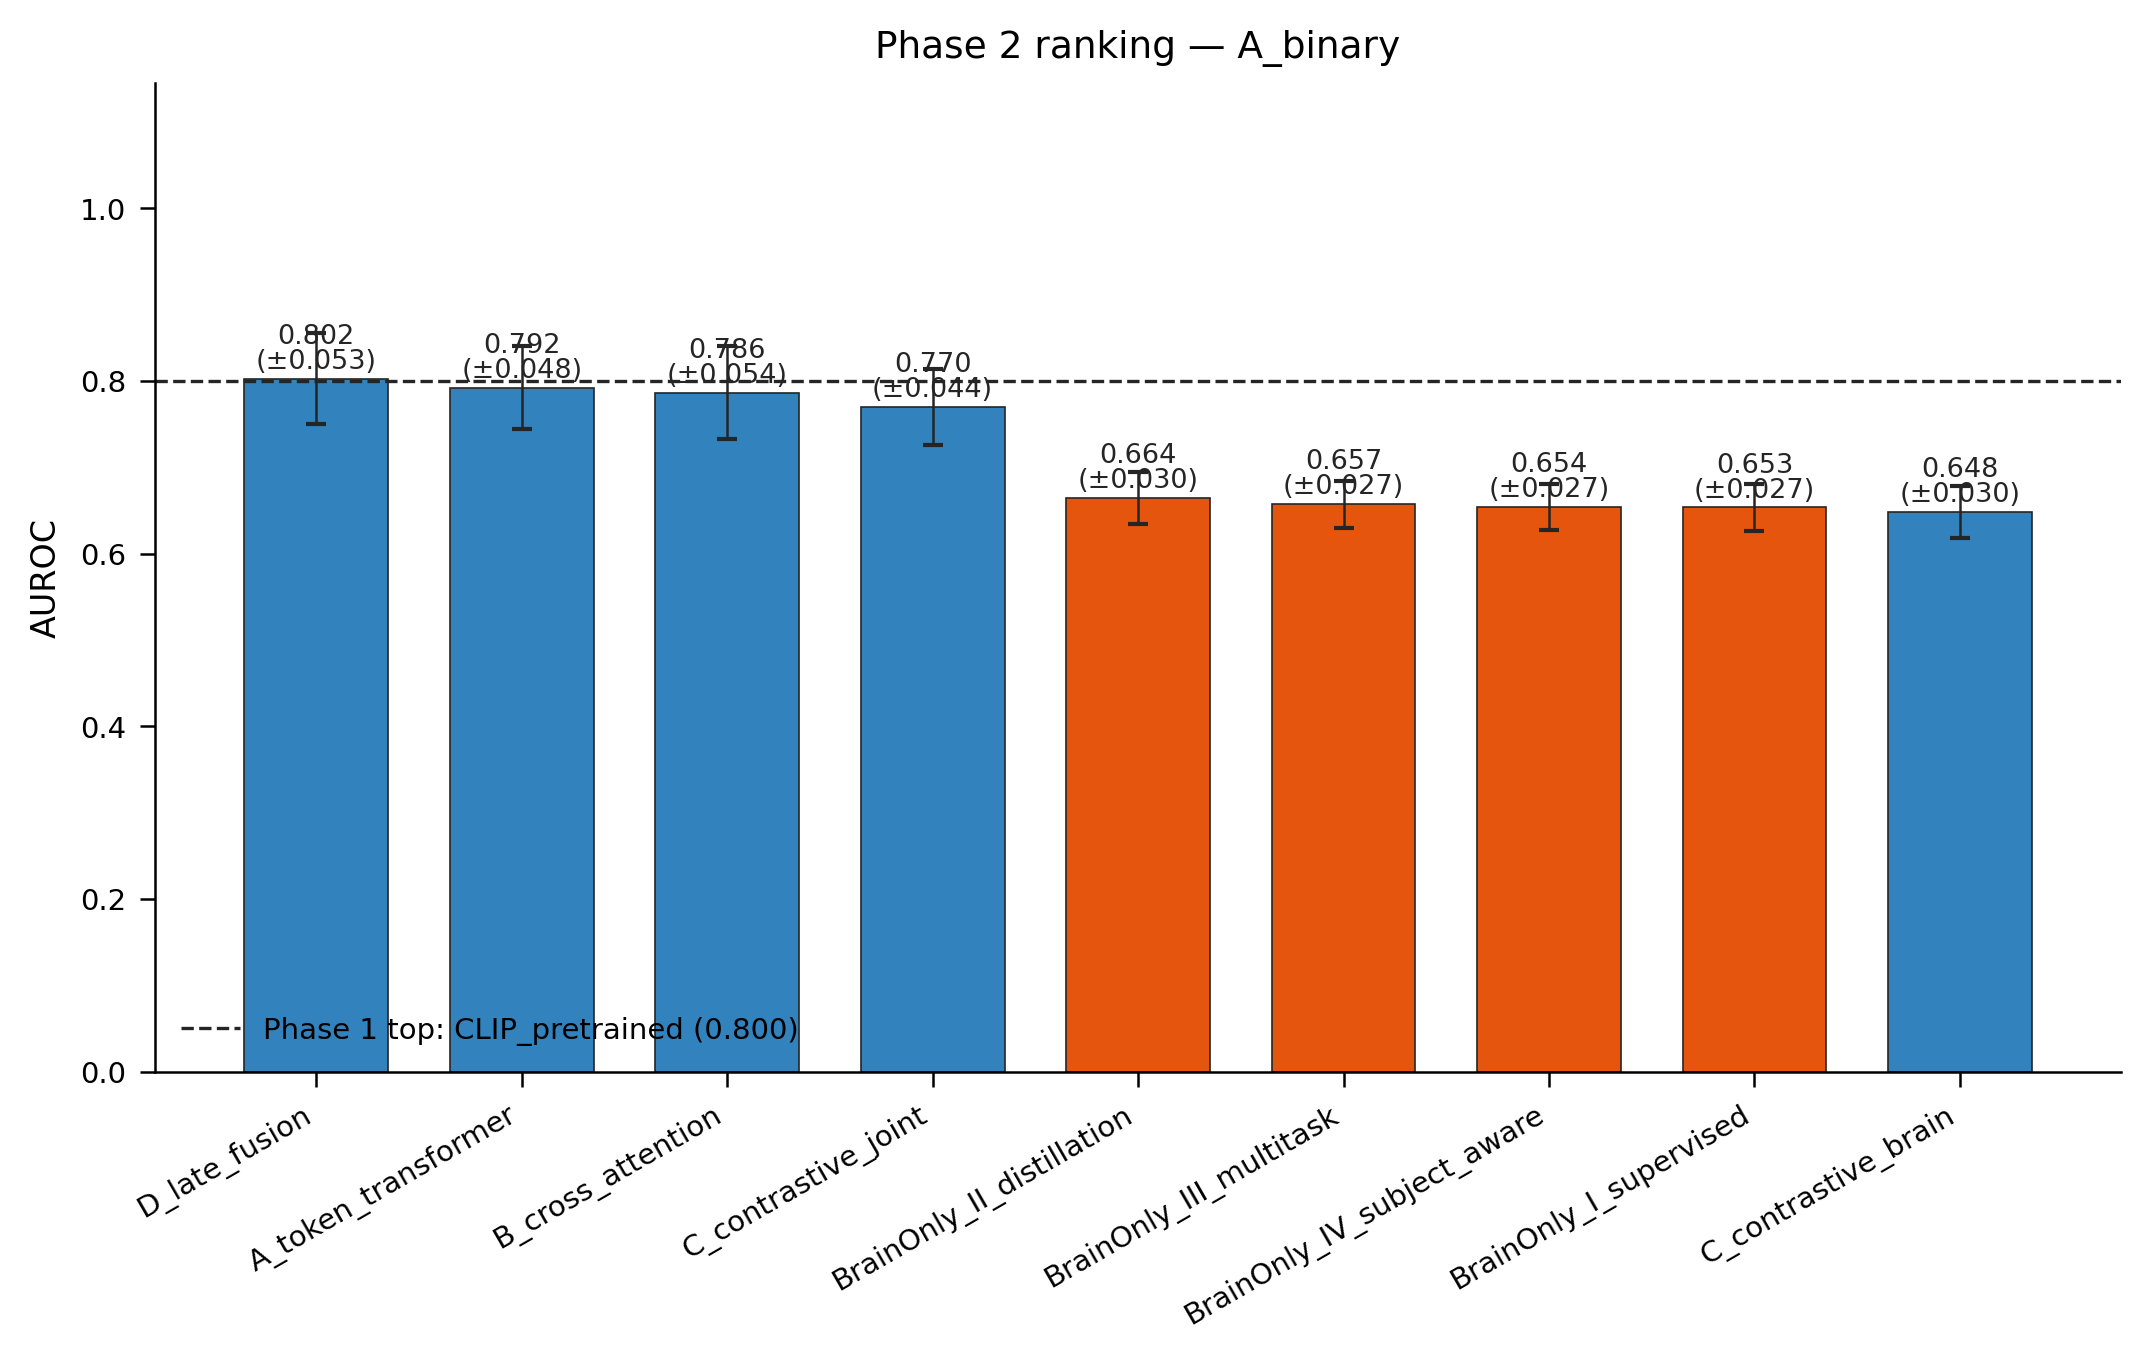
\includegraphics[width=\linewidth]{figs/ranking_A_binary.png}
  \caption{A\_binary, AUROC.}
\end{subfigure}

\vspace{4pt}

\begin{subfigure}{0.48\linewidth}
  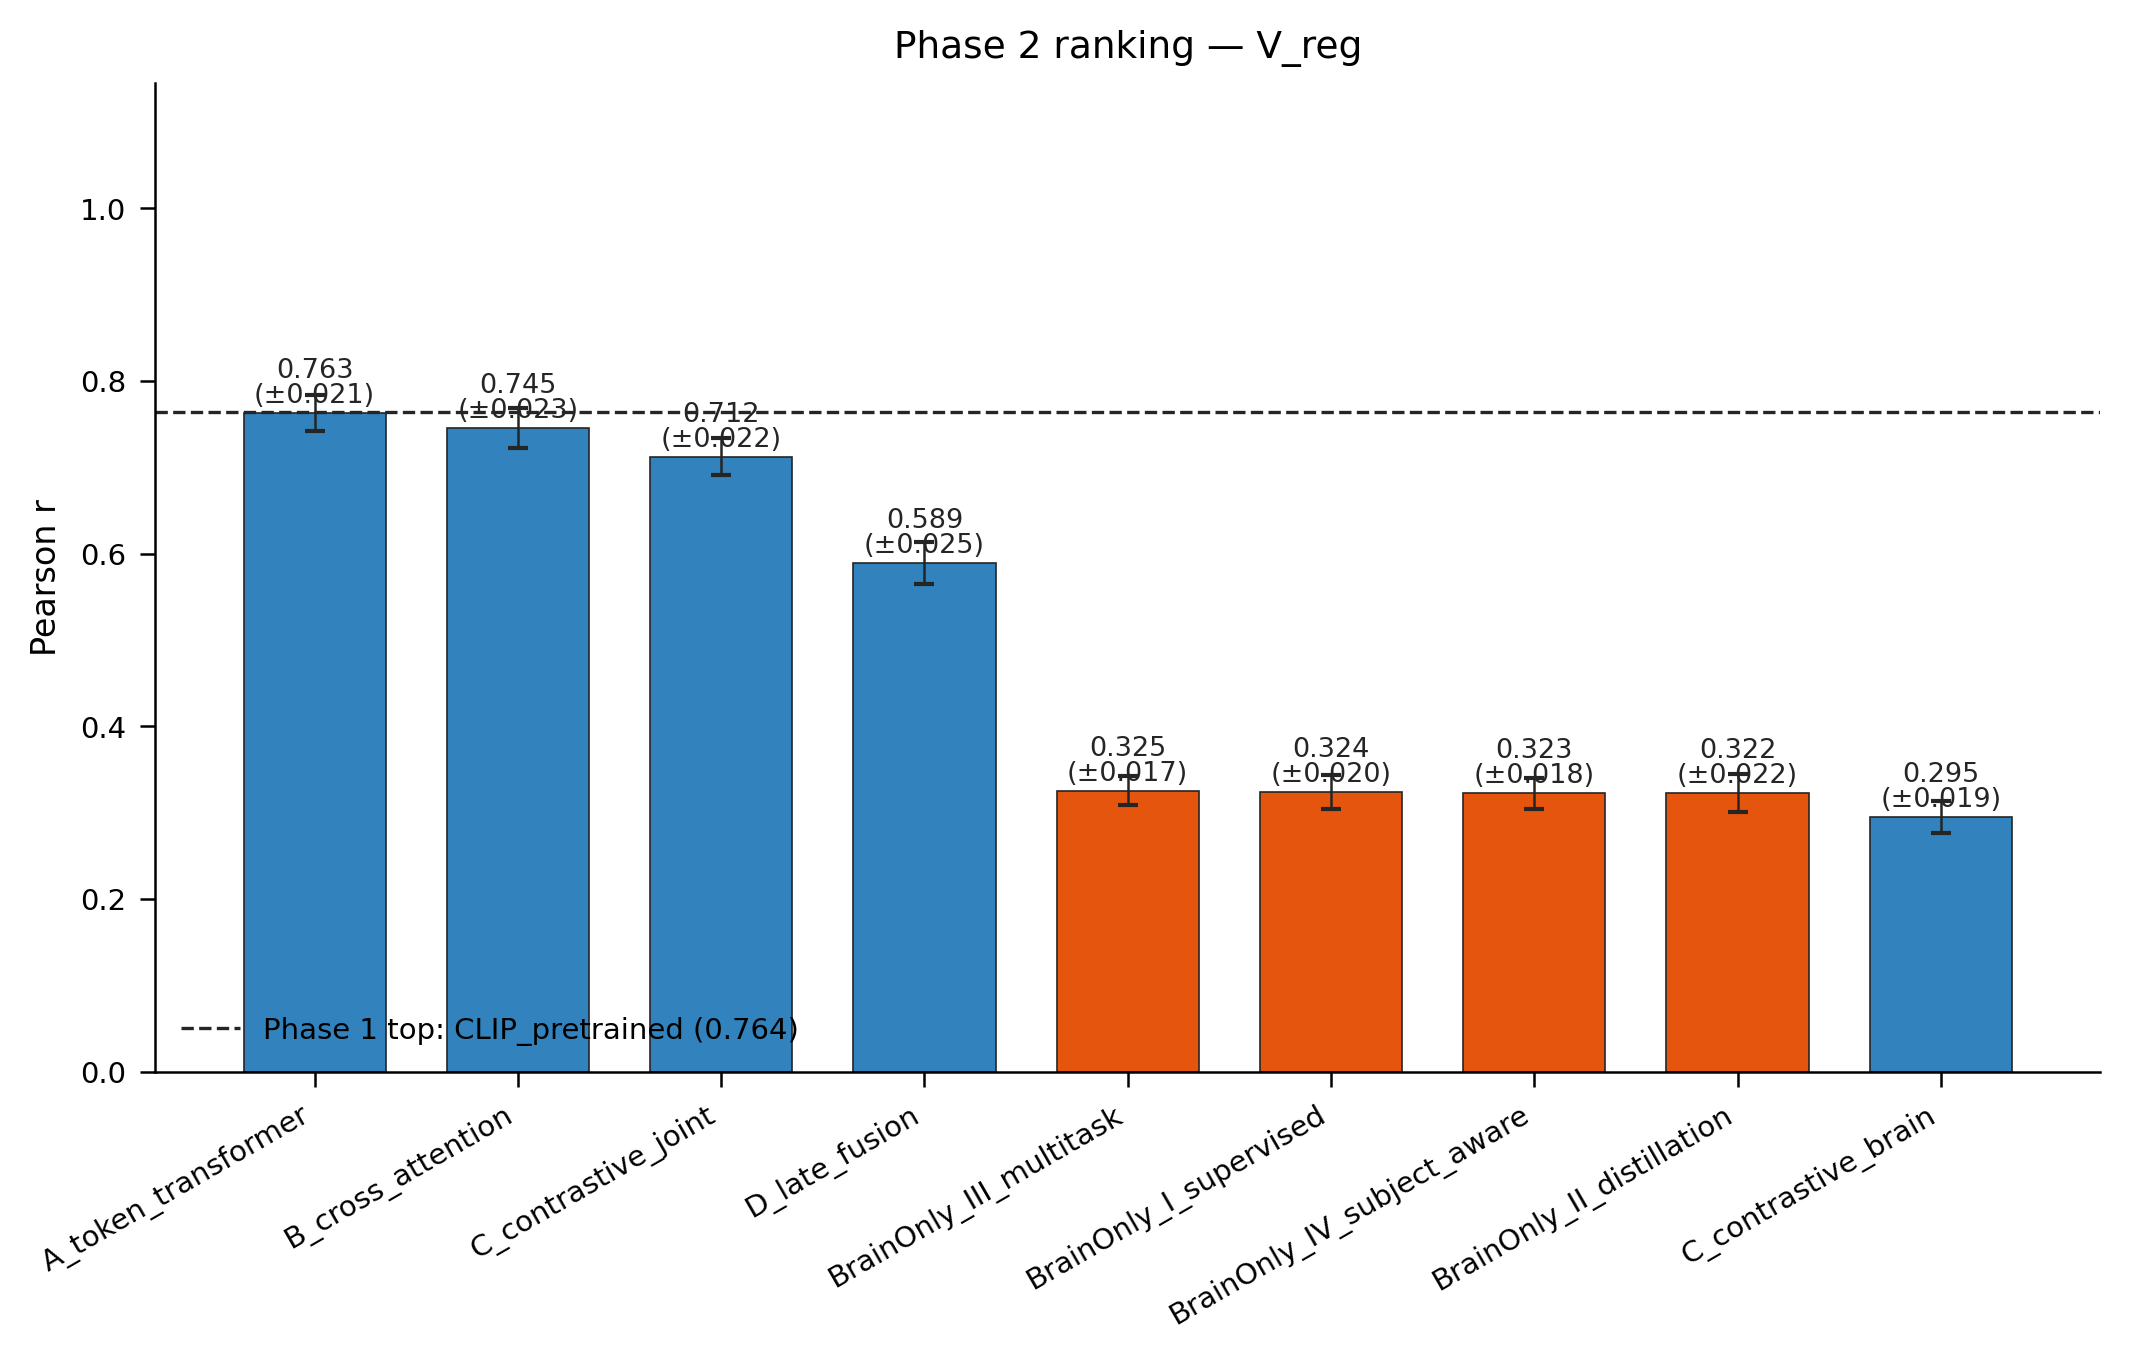
\includegraphics[width=\linewidth]{figs/ranking_V_reg.png}
  \caption{V\_reg, Pearson $r$.}
\end{subfigure}
\hfill
\begin{subfigure}{0.48\linewidth}
  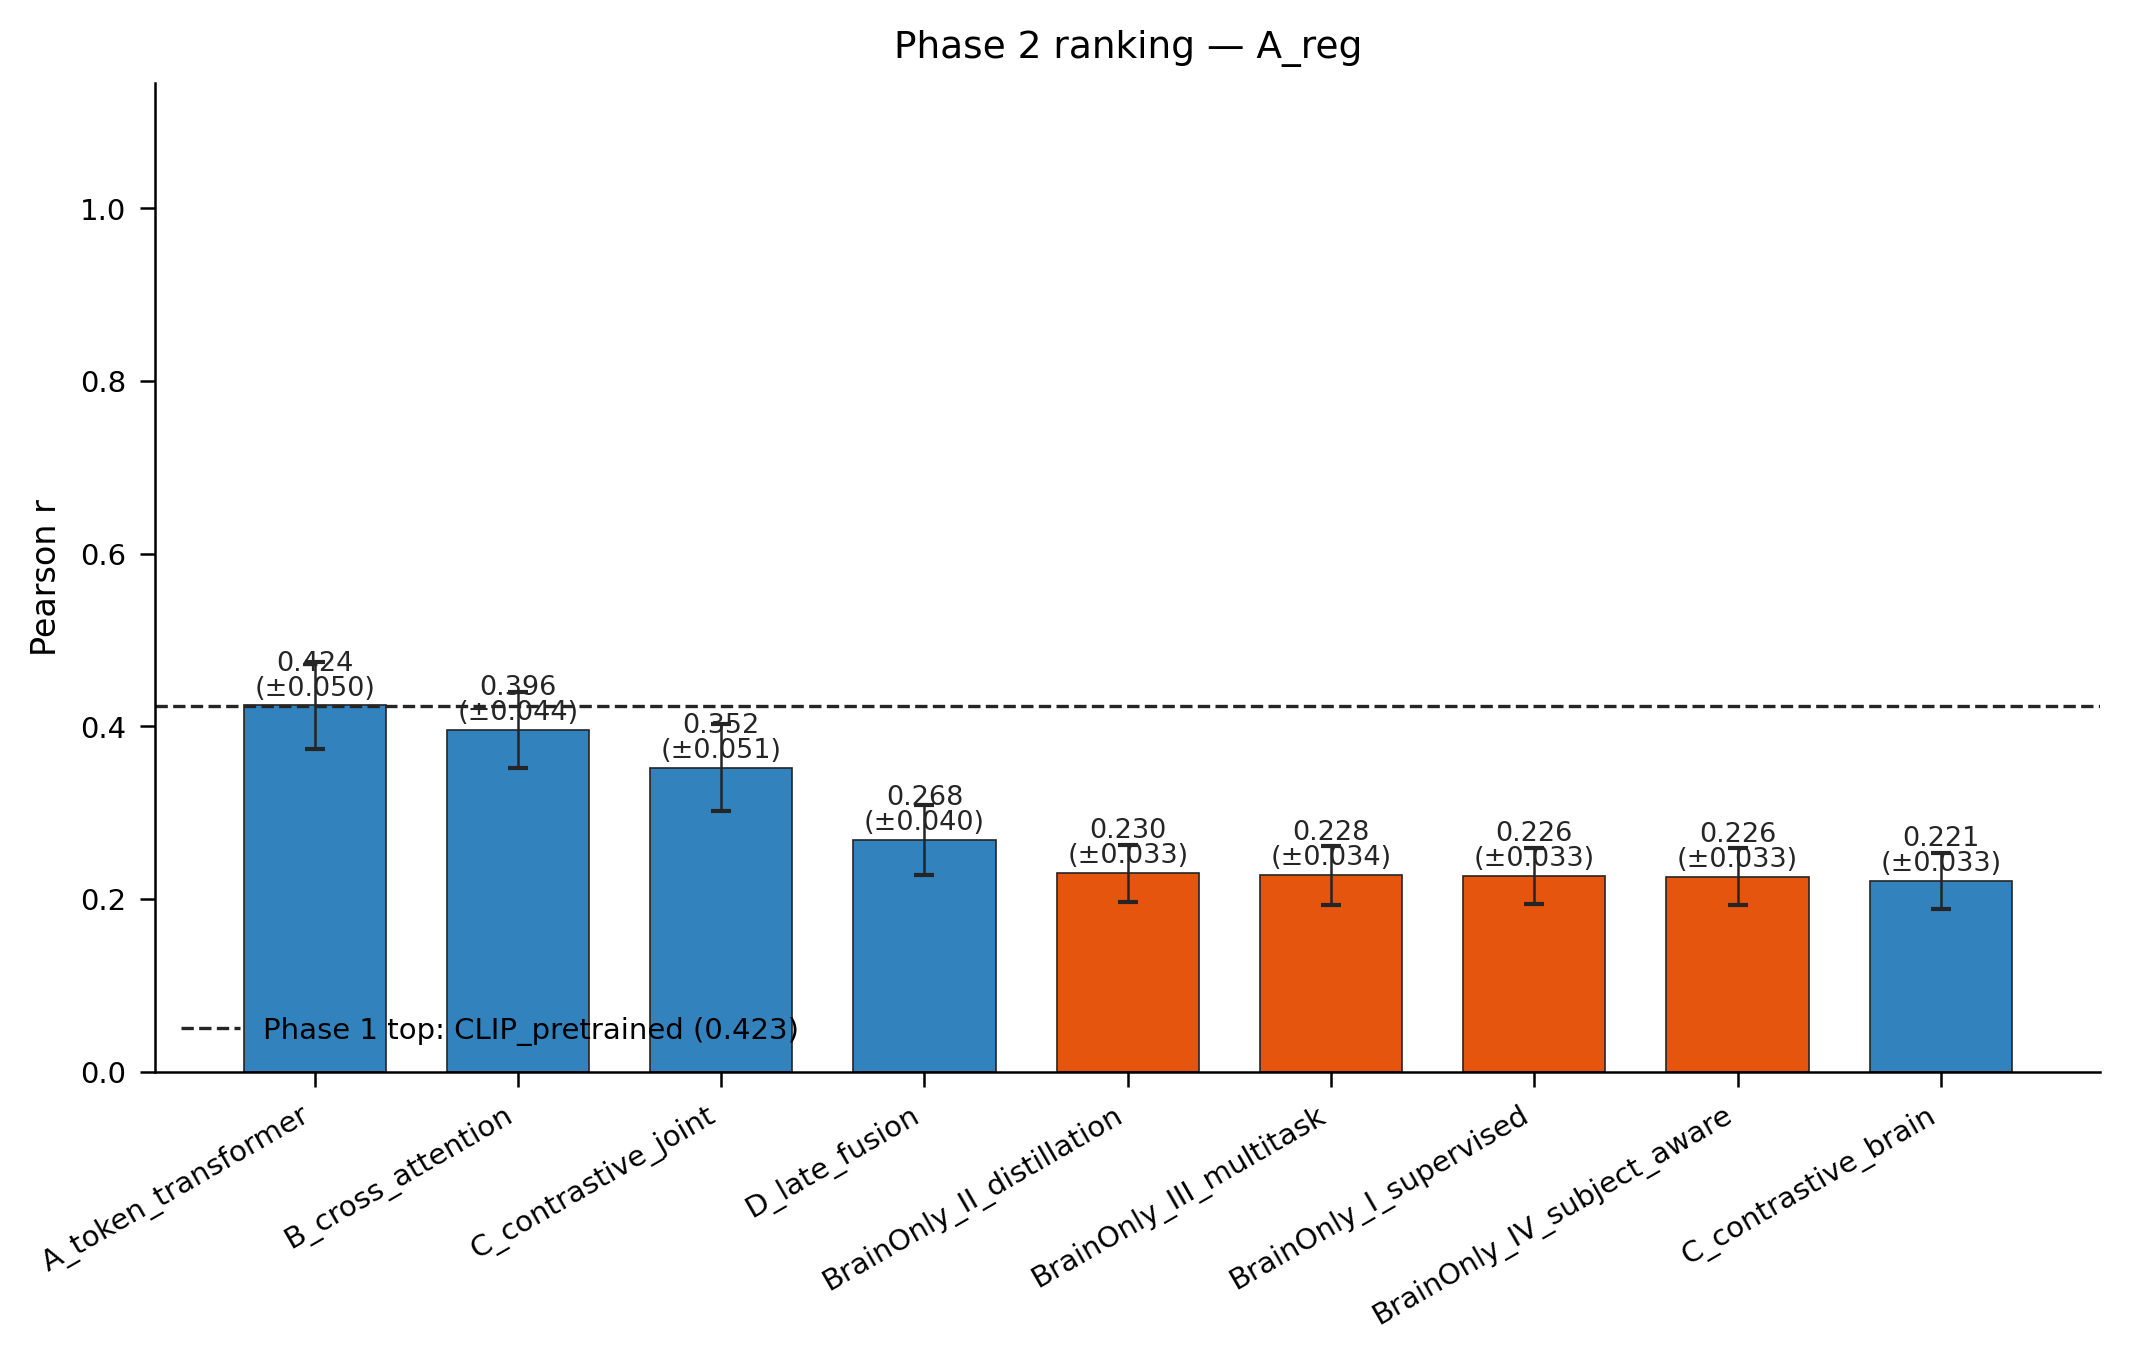
\includegraphics[width=\linewidth]{figs/ranking_A_reg.png}
  \caption{A\_reg, Pearson $r$.}
\end{subfigure}
\caption{Per-task ranking of all Phase 2 paradigms. Dashed line is Phase 1 top-overall
condition (CLIP frozen linear), dotted line is Phase 1 top brain-only condition.}
\label{fig:ranking}
\end{figure}

\subsection{Method by task heatmap}
Figure~\ref{fig:heat} reports the same numbers in heatmap form to expose the bimodal
structure (joint above, brain-only below) at a glance. The white horizontal line
separates the joint and brain-only groups.

\begin{figure}[h]
\centering
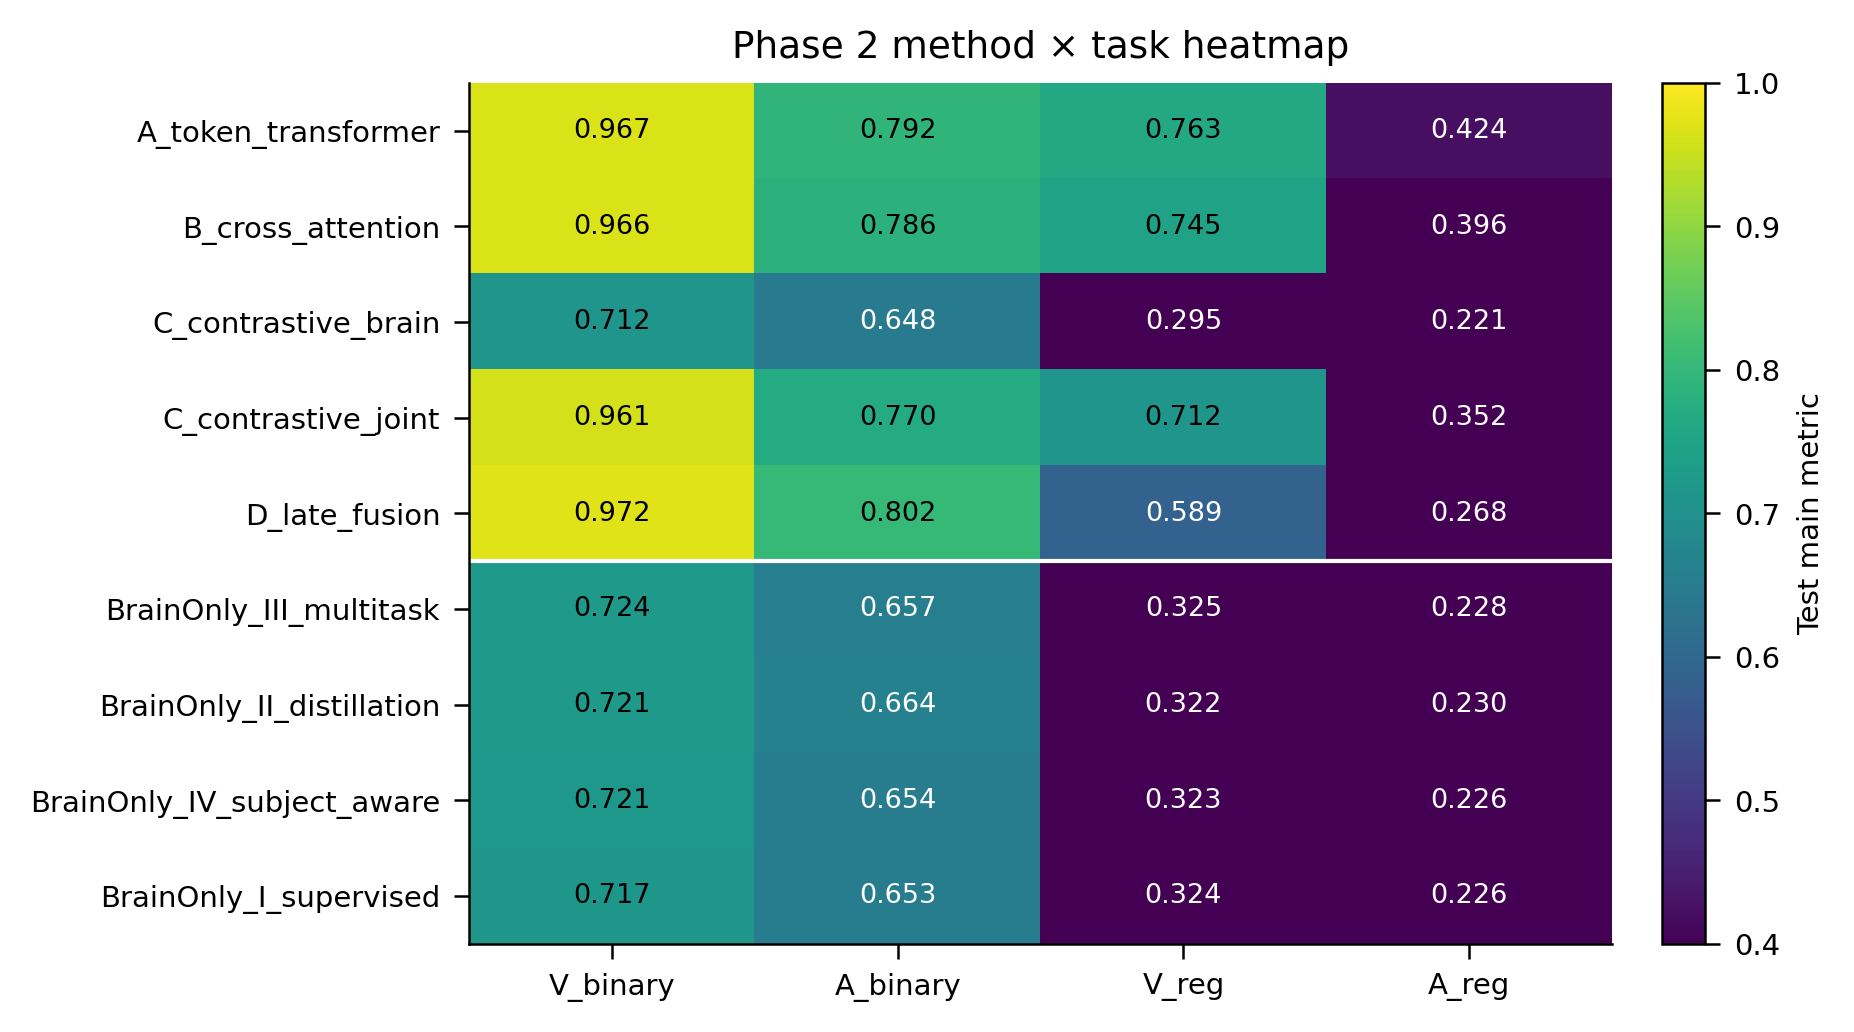
\includegraphics[width=0.74\linewidth]{figs/method_heatmap.png}
\caption{Paradigm by task heatmap. Rows are paradigms, columns are tasks. Cell label is
mean main metric across folds and seeds. The white horizontal line separates joint
(top) from brain-only (bottom).}
\label{fig:heat}
\end{figure}

\section{Discussion}
\label{sec:discussion}

\subsection{Brain-only paradigms do not move the frozen-probe ceiling}
The first result is a negative one. None of the four brain-only paradigms moves the
ceiling beyond what a plain linear or MLP probe achieved in Phase 1. Within-group spread
is below across-fold variability on every task, and the four paradigms are statistically
indistinguishable. This holds whether the auxiliary signal is a stronger video teacher
(Paradigm~II), an explicit reconstruction loss (Paradigm~III), or per-subject identity
(Paradigm~IV). With Brain-JEPA frozen as feature extractor and the brain side as the only
input, the small per-subject sample size and the limited emotion-relevant content of the
five-TR per-stimulus window appear to bind the achievable performance well below the
video-only number, and additional training signal at the head level does not relieve
this constraint. This is consistent with the Phase 1 conclusion that brain encoder
choice within the BFM family does not move the brain-only ceiling, and it suggests that
the constraint is not located at the head.

\subsection{Joint paradigms recover the video-only ceiling}
The second result is more positive. The four joint paradigms reach the video-only Phase
1 ceiling on three of four tasks and are within $0.003$ on the fourth. This is not a
claim that adding the brain feature improves over CLIP alone, since the deltas are
within across-fold variability. The relevant claim is symmetric. A joint model that
ingests brain alongside video does not lose performance relative to the video-only
baseline. This matters for the next phase of work because it means a joint architecture
is admissible as a substrate for follow-up questions such as subject-conditioned
variability and brain-attributable contribution analysis, neither of which is meaningful
on a model that throws away the brain side.

\subsection{Fusion architecture is task-dependent}
Within the joint group, the choice of fusion matters task by task. Late linear fusion
(Paradigm~D) is best on both binary tasks, and token-attention (Paradigm~A) is best on
both regression tasks. The margin between A and D on the regression tasks is large
($0.174$ Pearson $r$ on V\_reg, $0.156$ on A\_reg) and on the binary tasks is small
($0.0048$ AUROC on V\_binary, $0.0106$ on A\_binary). The likely interpretation is that
binary extreme-quartile prediction is dominated by a small number of discriminative axes
that a linear fusion already captures, while continuous regression benefits from
nonlinear interactions between brain and video features that the attention layers
explicitly model. We do not advocate a single preferred fusion for the project. We do
note that the late linear fusion baseline is closed form and runs in seconds per fold,
which makes it the natural sanity check that any future fusion design must clear.

\subsection{The contrastive brain branch erodes brain-side emotion information}
The third result concerns the contrastive paradigm. Paradigm~C trains brain and video
projections to be mutually predictive under an InfoNCE objective, with no emotion
supervision during alignment. Its joint readout is competitive with the other joint
paradigms, but its brain-only readout, which uses only the aligned brain branch, is the
weakest brain-only number on every task. The gap to the next-weakest brain-only paradigm
(supervised MLP, Paradigm~I) is $0.0042$ AUROC on V\_binary, $0.0049$ on A\_binary,
$0.0288$ Pearson $r$ on V\_reg, and $0.0054$ on A\_reg. Two of these are smaller than
the within-fold standard deviation but the V\_reg gap is meaningful in absolute terms.

A reasonable interpretation is that an InfoNCE objective that compresses the brain branch
into a representation maximally predictive of the video branch can discard
emotion-relevant brain information that the video branch does not carry, on the grounds
that aligned shared structure dominates the loss. This is a constructive negative result
for any future design that uses contrastive alignment as a preprocessing step for
brain-only inference. A supervised distillation objective (Paradigm~II), which preserves
the per-stimulus target on the brain side, does not show this regression.

\subsection{Implications for joint brain-video models}
For the BrainVLM follow-up, two implications carry. First, the joint architecture should
not be selected purely on classification performance. Late linear fusion would maximise
V\_binary and A\_binary, but token-attention is strictly preferred for regression tasks
and is the more honest substrate when both are evaluated jointly. Second, an alignment
objective should be added only as auxiliary supervision, not as the primary training
signal, and the brain branch should be regularised toward preserving emotion-relevant
content rather than purely toward video-prediction content.

\section{Limitations}
\label{sec:limits}

The Phase 2 numbers in this report fix the brain encoder to Brain-JEPA with the
\fefn{resting} initialisation and the video encoder to CLIP. Other Phase 1 frozen models
were not re-evaluated in Phase 2. The reason is computational. The same paradigm grid
was run for every brain and video combination in Phase 1, and re-running it for the full
cross-product in Phase 2 would have been a factor of 15 more expensive in seed-fold
units. The Brain-JEPA-plus-CLIP combination was chosen because it is the strongest
brain-only and video-only condition in Phase 1, so a paradigm that succeeds here is the
most informative test of paradigm effect. We do not claim that the paradigm rankings
generalise across choices of brain and video encoder.

The sample size remains small in absolute terms. Five subjects with $2185$ stimuli yield
$10925$ stimulus-subject observations under the regression protocol and $5675$ under the
binary protocol. The across-fold standard deviations reported throughout this paper are
on the same order as the paradigm-to-paradigm deltas within the brain-only group, which
is why we do not claim significance for any within-group ranking. The joint-to-brain-only
deltas are larger than across-fold variability by a factor of approximately five to
twenty, so those comparisons are robust.

The contrastive alignment was trained for a fixed number of epochs with a fixed
temperature initialisation and a fixed embedding dimension. We did not run an ablation
over these choices, so the brain-side erosion result should be read as an existence claim
for one specific configuration rather than as a general statement about contrastive
alignment in this regime.

\section{Conclusion}

We benchmarked eight downstream training paradigms on frozen Brain-JEPA and frozen CLIP
features under a single five-fold stimulus-stratified protocol on four naturalistic
emotion fMRI tasks. The four brain-only paradigms collapse onto the Phase 1 frozen-probe
ceiling regardless of training signal. The four joint paradigms recover the video-only
ceiling and, in two of four tasks, slightly exceed it. Within the joint group, late
linear fusion is best on the binary tasks and token-attention is best on the regression
tasks by a substantially larger margin. The contrastive paradigm, evaluated on its brain
branch alone after alignment, is the weakest brain-only paradigm on every task,
suggesting that an alignment objective without explicit emotion supervision can erode
brain-side information that is not shared with the video branch. Phase 3 of the project
will replace the frozen brain encoder with a learnable BrainVLM that ingests fMRI as
visual tokens into a Qwen3-VL language backbone. The Phase 2 results suggest that the
critical comparison for Phase 3 will be against the token-attention joint baseline on the
regression tasks, not against the late linear fusion on classification.

\appendix
\section{Reproducibility notes}
All Phase 2 result CSVs are saved at
\fefn{results/phase2/\{A,B,C,D\}/\{V\_binary,A\_binary,V\_reg,A\_reg\}.csv} for the joint
paradigms and at \fefn{results/phase2/brain\_only/\{I\_supervised,II\_distillation,
III\_multitask,IV\_subject\_aware\}/\{...\}.csv} for the brain-only paradigms.
Summary CSVs (per-task aggregate, joint vs brain-only, comparison against Phase 1) are at
\fefn{results/phase2/\_phase2\_benchmark\_per\_task.csv},
\fefn{\_phase2\_joint\_vs\_brainonly.csv}, and
\fefn{\_phase2\_vs\_phase1\_best.csv}. The unified analysis pipeline is
\fefn{code/analysis/phase2\_unified\_analysis.py}. Per-paradigm training entry points are
under \fefn{code/phase2/}.

\end{document}
